\subsection{Propriedades Matemáticas}

\begin{small}
\begin{itemize}
    \item \textbf{Conjectura de Goldbach:} Todo número par $n > 2$ pode ser representado como $n = a + b$, onde $a$ e $b$ são primos.

    \item \textbf{Primos Gêmeos:} Existem infinitos pares de primos $p$, $p + 2$.

    \item \textbf{Conjectura de Legendre:} Sempre existe um primo entre $n^2$ e $(n+1)^2$.

    \item \textbf{Lagrange:} Todo número inteiro pode ser representado como soma de 4 quadrados.

    \item \textbf{Zeckendorf:} Todo número pode ser representado como soma de números de Fibonacci diferentes e não consecutivos.

    \item \textbf{Tripla de Pitágoras (Euclides):} Toda tripla pitagórica primitiva pode ser gerada por $(n^2 - m^2, 2nm, n^2 + m^2)$ onde $n$ e $m$ são coprimos e um deles é par.

    \item \textbf{Wilson:} $n$ é primo se e somente se $(n-1)! \mod n = n - 1$.

    \item \textbf{Problema do McNugget:} Para dois coprimos $x$ e $y$, o número de inteiros que não podem ser expressos como $ax + by$ é $(x-1)(y-1)/2$. O maior inteiro não representável é $xy - x - y$.

    \item \textbf{Fermat:} Se $p$ é primo, então $a^{p-1} \equiv 1 \mod p$. Se $x$ e $m$ são coprimos e $m$ primo, então $x^k \equiv x^{k \bmod (m-1)} \mod m$.
          \textit{Euler:} $x^{\varphi(m)} \equiv 1 \mod m$. $\varphi(m)$ é o totiente de Euler.


    \item \textbf{Teorema Chinês do Resto:} Dado um sistema de congruências:
    \[
    x \equiv a_1 \mod m_1, \quad \ldots, \quad x \equiv a_n \mod m_n
    \]
    com $m_i$ coprimos dois a dois. E seja $M_i = \frac{m_1 m_2 \cdots m_n}{m_i}$ e $N_i = M_i^{-1} \mod m_i$. Então a solução é dada por: 
    \[
    x = \sum_{i=1}^{n} a_i M_i N_i
    \]
    Outras soluções são obtidas somando $m_1 m_2 \cdots m_n$.


    \item \textbf{Números de Catalan:} Exemplo: expressões de parênteses bem formadas. $C_0 = 1$, e:
    \[
    C_n = \sum_{i=0}^{n-1} C_i C_{n-1-i} = \frac{1}{n+1} \binom{2n}{n}
    \]


    \item \textbf{Bertrand (Ballot):} Com $p > q$ votos, a probabilidade de sempre haver mais votos do tipo $A$ do que $B$ até o fim é:
    $ \frac{p - q}{p + q} $
    Permitindo empates: 
    $\frac{p + 1 - q}{p + 1}$. Multiplicando pela combinação total $\binom{p + q}{q}$, obtém-se o número de possibilidades.

    
    \item \textbf{Linearidade da Esperança:} $E[aX + bY] = aE[X] + bE[Y]$

    \item \textbf{Variância:} $\text{Var}(X) = E[(X - \mu)^2] = E[X^2] - E[X]^2$

    \item \textbf{Progressão Geométrica:} $S_n = a_1 \cdot \frac{q^n - 1}{q - 1}$

    \item \textbf{Soma dos Cubos:} $\sum_{k=1}^{n} k^3 = \left( \sum_{k=1}^{n} k \right)^2$

    \item \textbf{Lindström-Gessel-Viennot:} A quantidade de caminhos disjuntos em um grid pode ser computada como o determinante da matriz do número de caminhos.
    
    \item \textbf{Lema de Burnside:} Número de colares diferentes (sem contar rotações), com $m$ cores e comprimento $n$:
    \[
    \frac{1}{n} \left(m^n + \sum_{i=1}^{n-1} m^{\gcd(i, n)} \right)
    \]

    \item \textbf{Inversão de Möbius:}
    \[
    \sum_{d \mid n} \mu(d) = \begin{cases}
    1, & n = 1 \\
    0, & \text{caso contrário}
    \end{cases}
    \]

    \item \textbf{Propriedades de Coeficientes Binomiais:}
    % \begin{align*}
    % \end{align*}
    % \vspace{-2pt}
    \begin{alignat*}{2}
        \binom{N}{N - K} &= \frac{N}{K} \binom{N - 1}{K - 1} = \binom{N}{K}   &\\
        \sum_{k=0}^{m} (-1)^k & \binom{n}{k} = (-1)^m  \binom{n - 1}{m}       &\\
        \sum_{k=0}^{n} \binom{n}{k} &= 2^n     ,                              &
        \sum_{k=0}^{n} k \binom{n}{k} = n \cdot 2^{n - 1}                      \\
        \sum_{m=0}^{n} \binom{m}{k} &= \binom{n+1}{k+1}  ,                    &
        \sum_{k=0}^{n} \binom{n-k}{k} = F_{n+1}                                \\
        \sum_{k=0}^{m} \binom{n + k}{k} &= \binom{n + m + 1}{m}  ,            &
        \sum_{k=0}^{n} \binom{n}{k}^2 = \binom{2n}{n}
    \end{alignat*}

    \item \textbf{Triângulo de Pascal} \\[0.5ex]
    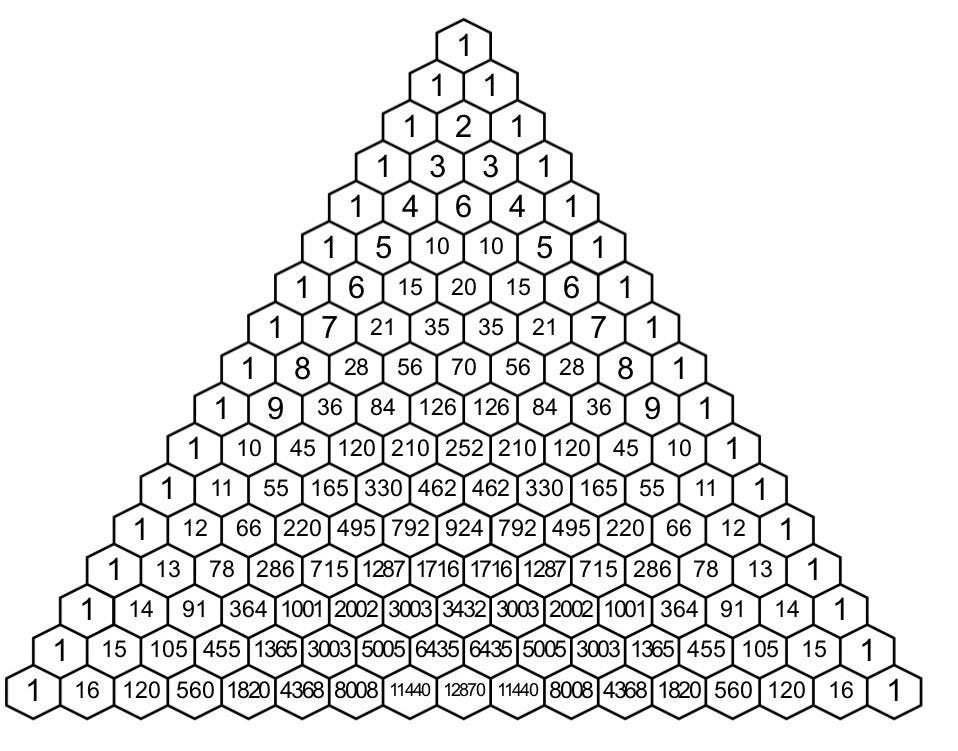
\includegraphics[width=\linewidth]{math/pascal}

    \item \textbf{Identidades Clássicas:}
    \begin{itemize}
        \item \textbf{Hockey-stick:} $\sum_{i=r}^{n} \binom{i}{r} = \binom{n+1}{r+1}$
        \item \textbf{Vandermonde:} $\binom{m+n}{r} = \sum_{k=0}^{r} \binom{m}{k} \binom{n}{r-k}$
    \end{itemize}

    \item \textbf{Distribuições de Probabilidade:}
    \begin{itemize}
        \item \textbf{Uniforme:} $X \in \{a, a+1, \dots, b\}$, $E[X] = \frac{a + b}{2}$
        \item \textbf{Binomial:} $n$ tentativas com probabilidade $p$ de sucesso:
        \[
        P(X = x) = \binom{n}{x} p^x (1 - p)^{n - x}, \quad E[X] = np
        \]
        \item \textbf{Geométrica:} Número de tentativas até o primeiro sucesso:
        \[
        P(X = x) = (1 - p)^{x - 1} p, \quad E[X] = \frac{1}{p}
        \]
    \end{itemize}

\end{itemize}
\end{small}
% credits: https://github.com/gabrielpessoa1/ICPC-Library/